\documentclass[a4paper]{article}
\usepackage[utf8]{inputenc}
\usepackage[english]{babel}

\usepackage{amsmath}
\usepackage{amsfonts}
\usepackage{amssymb}
\usepackage{graphicx}
\usepackage{fancyhdr}
\usepackage{moreverb}
\usepackage{listings}
\usepackage{courier}
\usepackage{qtree}
\usepackage[normalem]{ulem}
\usepackage{color}
\usepackage{comment}
\usepackage{float}
\usepackage{enumitem}
\usepackage{etoolbox}
\usepackage{scrextend}

\newcommand{\setR}{\mathbb{R}}
\newcommand{\setZ}{\mathbb{Z}}
\newcommand{\setN}{\mathbb{N}}
\newcommand{\setF}{\mathbb{F}}
\newcommand{\lra}{\leftrightarrow}
\newcommand{\Lra}{\Leftrightarrow}
\newcommand{\ra}{\rightarrow}
\newcommand{\Ra}{\Rightarrow}
\newcommand{\tbf}[1]{\textbf{#1}}
\newcommand{\tit}[1]{\textit{#1}}
\newcommand{\tsc}[1]{\textsc{#1}}
\newcommand{\tsf}[1]{\textsf{#1}}
\newcommand{\tsl}[1]{\textsl{#1}}
\newcommand{\ttt}[1]{\texttt{#1}}
\newcommand{\subsubsubsection}[1]{\tbf{#1}}
\newcommand{\makeline}[1]{\noindent\makebox[\linewidth]{\rule{#1}{0.5pt}}}
\newcommand{\marginwidth}{0.5cm}

\makeatletter
\pretocmd{\section}{\addtocontents{toc}{\protect\addvspace{1\p@}}}{}{}
\pretocmd{\subsection}{\addtocontents{toc}{\protect\addvspace{0\p@}}}{}{}

\lstset{	numbers=left,
		numberstyle=\footnotesize\ttfamily,
		numbersep=8pt,
		frame = single,
		basicstyle=\ttfamily,
		keywordstyle=\bfseries,
		commentstyle=\color{green},
		showstringspaces=false,
		morekeywords={include, printf, int, if, else, sizeof, void}
		}

\renewcommand{\headrulewidth}{0pt}

\title{Assisting Fuzzing with Concolic Execution}
\author{Søren Lund Jensen}
\begin{document}

\maketitle %TODO ændr til en flottere forside

\tableofcontents

\newpage
\section{Abstract}
\label{sec:Abstract}

\newpage
\section{Introduction and concept}
\label{sec:Intro}
An ever-present danger in today's society is memory corruption vulnerabilities in software, be they use of uninitialized memory, using dangling null-pointers, buffer overflow, memory leaks, or a fifth, sixth- or seventh vulnerabilities. An attacker could, did he know of these vulnerabilities, exploit them in order to access confidential informations, create DOS-attacks or other and as computer processing and connecting continues to be on the rise, playing a major role in present day, patching these vulnerabilities has to be a priority. This, of course, cannot be done without first discovering said bugs. 

Memory corruption bugs are often-case virtually untraceable, as only specific input combinations may trigger them, or the fact that they may appear under very unusual conditions, which makes it very hard to discover, or in some cases, even reproduce them. Add thereto, the fact, that the memory corruption's effect may manifest itself far away from its source, it can also be hard to even correlate these two, once a bug has been discovered.

A variety of tools exists, with the purpose of bug-discovery, but as the bugs are often very specific, and/or wide-spread, creating a silver bullet is hard, if not impossible. Many vulnerabilities are discovered manually, however, this solution is not scalable, as software applications generally increase in size and complexity. A handful of tools exist, including fuzzers and symbolic execution engines. These do, however have, in the worst cases, deal-breaking flaws, working against them, and their usefulness.

In late 2015, early 2016, The Defence Advanced Research Projects Agency (DARPA) hosted the 2016 Cyber Grand Challenge, with the theme of promoting and advancing automated computer security techniques, ranging from bug-detection to bug-squashing to hacking - all without interference from the teams who've created the software. Among the three teams, qualified for the final event, taking place August 2016 was Team Shellphish, who had created the Driller project: an extended version of American Fuzzy Lop, augmented by the concolic execution-engine, known as angr.

The idea behind this technology is to, through combining AFL with angr, mitigate as many of each of their respective drawbacks, while simultaneously utilizing many of their advantages - even create new symbiotic advantages.
\subsection{Problem statement}
\label{sec:problem}
Does Driller display a significant difference, in terms of running time and bugs/ vulnerabilities found, when compared to "regular" fuzzing, or is the technology?

Alternatively, is Driller suffering from being too narrowly engineered, as to better fit the kind of test-binaries given by DARPA, and so non-usable in real day intrusion-combating?
\newpage
\section{Team Shellphish}
\label{sec:Shellphish}
%TODO 1: Skriv section. 2: tænkt måske lidt som en pre-acknowledgement
\section{American Fuzzy Lop}
\label{sec:AFL}
This program works by feeding random input to a program, at a very high rate, some of which will hit specific vulnerabilities in said input-program. Every input fed is logged, and upon vulnerability-hit, AFL logs the input-ID. Hereafter information about where the vulnerability occurred, and which input triggered it is gatherable, based on input ID.

An advantage, as well as a drawback of most fuzzers, hereunder AFL is its execution method, which is to be as non-invasive as possible, as to prioritize speed before complexity handling. This means that AFL does not analyse a fuzzed application, but instead directly executing the application with random input, which is immensely faster than mutating qualified input variables, based on an application analysis.
\subsection{Features of AFL}
\label{sec:FeaturesAFL}
AFL implements a variety of features, to enhance its efficiency. In this section, I will list some of the key features, offered.\\
\subsubsubsection{Genetic Fuzzing}
\begin{addmargin}[\marginwidth]{0cm}
When stating that the AFL fuzzing engine relies on executing applications with inputs at absolute random, one is not totally correct. This is due to the technique known as 'Genetic Fuzzing'. Genetic fuzzing means that the engine generates - \tit{unique} - inputs at total random. Simplified, this means that the current input, that AFL is generating cannot be the same as a previously generated input.
\end{addmargin}
\subsubsubsection{Stable Transition Tracking}
\begin{addmargin}[\marginwidth]{0cm}
AFL views the union of source and destination as a tuple of it's destination blocks. These tuples are prioritised, meaning that the tuples that cause the most different execution, compared to previous executions, are chosen first for future input generation.
\end{addmargin}
\subsubsubsection{Loop Bucketization}
\begin{addmargin}[\marginwidth]{0cm}
For a symbolic execution engines and fuzzers alike, loops are complicated to handle, as looping potentially offers an added layer of complexity. The AFL fuzzer makes the following contortions, in order to avoid looping's added complexity, and path space requirements:
When AFL detects that a triggered path contains a loop, it logs the executed loop iterations and compares this with previous inputs. The paths are grouped, based on the amount of iterations, and hereafter only \tit{one} path in a group is selected for further fuzzing. Using this the execution time of executing low loop-including paths is reduced to $O(log(N))$, as opposed to $O(N)$, if every single path should be discovered.
\end{addmargin}
\subsubsubsection{De-randomization}
\begin{addmargin}[\marginwidth]{0cm}
When AFL meets a random number, mutating one input value might not yield the same result, as mutating the same input value immediately after. Because of this, AFL features de-randomization, which allows for it to force randomized variables, to consistently use a specific seed, which in turn allows for consistent input/output-relations.
\end{addmargin}
\newpage
\subsection{Limitations of AFL}
\label{sec:LimitsAFL}
Because of the union of the above techniques and its general nature, AFL is able to quickly discover a wide selection of general vulnerabilities, meaning vulnerabilities, that are triggered by some \tit{kind} of input. When vulnerability-triggers move past general input, and into the territory of general input AFL can potentially fall seriously behind.
\begin{lstlisting}[caption=A program that is difficult to fuzz, label=diffToFuzz, captionpos=b]
int main(void)
{
    int x;
    read(0, &x, sizeof(x));
    
    if (x == 0x12345678){
        vulnerability();
    }else{
         ...
    }
}
\end{lstlisting}
A generic example of this can be seen in Listing \ref{diffToFuzz}. This describes a program, that takes an input $x$ from a user. If, and only if, $x$ evaluates to $0x12345678$ the program will fail, as a vulnerability has been triggered, and as so, at each command, executed by the fuzzer, the frequency, and by extension, the chance of discovering the bug, is $1$ in $2^{32}$. Furthermore, as the AFL lacks the ability to produce new paths within this specific program lacks, it's instrumentation falls short, and AFL is reduced to randomly mutating non-instrumented input.
\section{Symbolic Execution}
\label{sec:SymEx}
Symbolic execution, or symbolic evaluation, is a way of program analysis, designed in order to determine the different ways said program can be executed, and which type of input causes it. Instead of executing actual values, to determine this, an interpreter assigns symbolic values to the input variables. The symbolic used to visualise how the program will execute, based on what \tit{kind} of input it will be fed.
\subsection{Features of Symbolic Execution}
\label{sec:FeaturesSymEx}
As symbolic execution relies on analysing input, instead of mindlessly executing input, it is able to detect specific inputs which, in this case, cause the application to crash. See Listing \ref{diffToFuzz} as an example. A symbolic execution engine will analyse it's functions, and generate the following tree:\\
\centerline{\Tree [.$\emptyset$ [. $x==0x12345678$ $\neg(x==0x12345678)$ ] ]}
\newpage
\noindent Another advantage of symbolic execution is the ability to invalidate sections input.
\begin{lstlisting}[caption=Example of Symbolic Execution, label=symExExample, captionpos=b]
int main(void)
{
    int x;
    read(0, &x, sizeof(x));
    
    if (x > 0x01){
        ...
    }else{
        ...
    }
    if x > 0x10){
        ...
    }else{
        ...
    }
}
\end{lstlisting}
In Listing \ref{symExExample} above, for example, the input $y$ is evaluated. A symbolic execution engine will analyse Listing \ref{symExExample}'s formulae, to find that $y$ will either assume a value greater than $0x01$ or not greater than $0x01$. Furthermore $y$ will either assume a value greater, or not greater than $0x10$, however greater than $0x10$ cannot occur, if $y$, at the same time was not greater than $0x01$. This will produce the following tree:\\
\centerline{
	\Tree [.$\emptyset$
			[.$y>0x01$ 
				[. $y>10$ 
				   $\neg(y>0x10)$
				]
			]
			[.$\neg(y>0x01)$
				[. \xout{$y>0x10$} 
				   $\neg(y>0x10)$ 
				]
			]
		]
}
Because of this trait, symbolic execution's relevance to the experiment is further heightened, as this allows for AFL to exclude certain value-ranges, when mutating input.
\subsection{Limitations of Symbolic Execution}
\label{sec:LimitsSymEx}
\subsubsubsection{Program-Dependent Efficiency}
\begin{addmargin}[\marginwidth]{0cm}
The advantage of having a symbolic execution-engine analyse paths, as opposed to input, is not present in all programs. If some inputs take the same paths in a program, the difference in analysing the inputs instead of paths, is vanishingly small.
\end{addmargin}
\subsubsubsection{Environment Interactions}
\begin{addmargin}[\marginwidth]{0cm}
Often programs interact with their environment, such as executing system calls and/or receiving signals. This becomes a problem when these environment factors are not under the control of the symbolic execution tool, as the tool is not able to determine branching of a program, when it has insufficient data concerning input.
\end{addmargin}
\subsubsubsection{Path Explosion}
\begin{addmargin}[\marginwidth]{0cm}
The last, and possibly biggest drawback in symbolic execution engines is the path explosion problem. This problem is caused by a program that is containing loops, which causes the amount of path to grow exponentially. In theory the path amount can even become infinite, because of unbound loops. This problem is near-not-existing in small programs, however it often scales faster than the symbolically executed program scales, rendering symbolic execution virtually useless for testing medium to large applications.
\end{addmargin}
\section{angr: The Concolic Execution Engine}
\label{sec:angr}
angr is a binary analysis framework, engineered modularly to be as versatile and composable as possible. Because of this, angr's use has potential to span wide, within the subject of binary analysis. Consider, for instance, just these few, but broad, uses of angr:
\begin{itemize}
	\item angr can be used as a dynamic symbolic execution engine, which combined with value set analysis, which allows to resolve bounds on symbolic variables.
	\item angr can be used as a static analysis engine, which also uses concolic tracing, in order to prove that detections are not false positives.
	\item angr can be used as a concolic tracer, along with a fuzzer, such as AFL, in order to allow for fully automatic bug discovery, such as what was done with Driller.
\end{itemize}
Driller would receive no benefit from invoking a regular symbolic execution engine, when stuck, as AFL cannot mutate input, based on symbolic values. Instead, using angr, an execution engine with the ability to mutate concrete values, based on the values found in the previous symbolic analysis-step.

angr, based on Mayhem \cite{Mayhem}, mutates concrete values via a four steps long algorithm. The steps can be broken down into the following:
\begin{itemize}
	\item[1] The input (i.e. binary code) is translated into Valgrind's VEX \cite{VEX} representation in order to determine the symbolic states of the binary code.
	\item[2] Symbolic values are set in place of all non-constant variables, such as user-defined input, randomized input, environment-dependant input, etc. Constant values are represented with the same concrete values, by which they are represented in the program.
	\item[3] The values are, by execution, given constraints set up by the binary environment, as well as the concrete values described in step 2.
	\item[4] When the program reaches a new path or state, input values, which drive the program to that state is generated, based on the constraints described step 2.
\end{itemize}
At any point after the algorithm has run, the gathered concrete values can be fed to the binary code, which will trigger the binary to produce an output similar to the one, that a corresponding symbolic value has generated.
\subsection{Diversity}
\label{sec:Diversityangr}
One of the design goals for angr has been to tailor it to be as diverse as possible. This was done, as angr was not only designed for its use in Driller, but was meant to be reusable, by team Shellphish, as well as any other security enthusiast out there. Because of this, angr was aimed towards support for ARM and MIPS processors, as well s 64-bit processors, instead of the 3-bit processors of yesteryear.

In the same spirit as the above mentioned cross-architecture support, angr also has to be able to support input, stemming from multiple platforms. This functionality is provided by the binary loader, called CLE, which is described in further detail in section \ref{sec:binaryLoader}.

Furthermore, when creating angr, team Shellphish did so, not only to further their odds in the DARPA CGC, but also to advance the bug-discovering community, and as a result of this, the tool is available as a fully editable open sourced program, completely free to use for any non-commercial use.
\subsection{The Binary Load Sub-Module}
\label{sec:binaryLoader}
When angr loads binaries into the application, it is handled by the binary load module, by the name of CLE. CLE is named, jokingly and recursively as an abbreviation for the sentence 'CLE Loads Everything'.

CLE is, as the point of departure, designed to work in the same way as GNU LD does with ELF binaries. This means that CLE does not necessarily load all the information in a binary, as some of this may be stripped or corrupted. When this happens, the ignored information is encompassed in a Project class. The rest of the information is stored in a Loader class, an in turn the CLE loader is representing a conglomerate of binaries, loaded by CLE, which, after being loaded, is mapped onto a single memory space. CLE has a subclass/ loader for each file type.

Currently, CLE offers support through its backends for PE, CGC, and both ordinary and core dump ELF files. Furthermore, CLE is able to load binaries with IDA, as well as loading files int flat address spaces. Which backend a binary file should use is auto-detectable for all, except the binaries, being loaded into flat images, which do need to be specified.
\section{Driller: Concolic Execution-Assisted Fuzzing}
\label{sec:Driller}
The core assumption, when team Shellphish designed Driller, was that 99+ \% of input could be divided into two categories: \tit{general} input, spanning over a broad pallet of values and \tit{specific} input, which is only able to take on a select few forms. Further chasing this assumption, the Driller approach emerges, which sees binaries as a collection of compartments. A representation of this can be seen in Figure \ref{Compartments} below:
\begin{figure}[H]
	\centering
	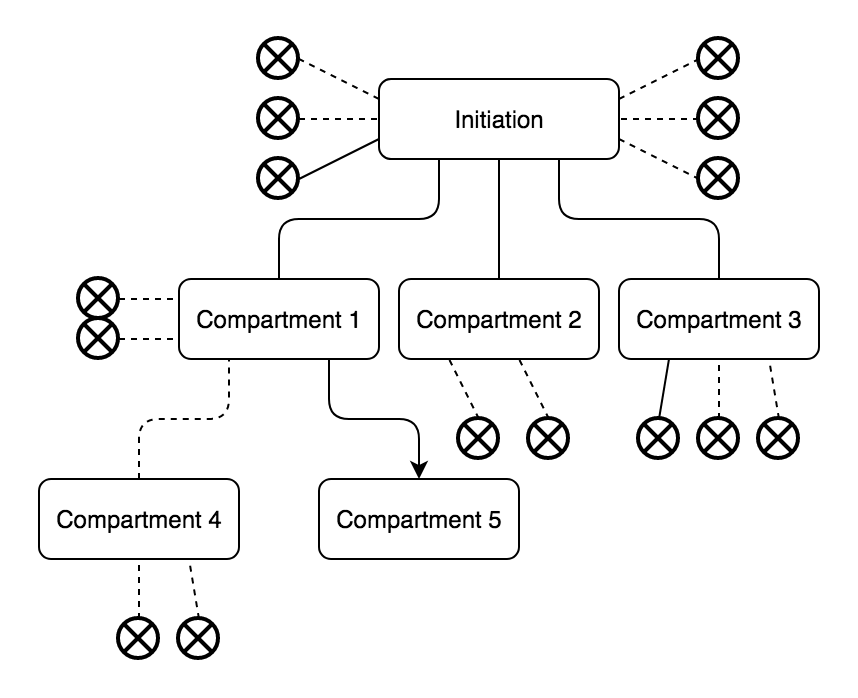
\includegraphics[width=0.5\textwidth]{Compartments}
	\caption{A graphic representation of binary compartments}
	\label{Compartments}
\end{figure}
\noindent
In Figure \ref{Compartments}, a path found by executing concolically is represented by a solid line, and a path found by means of fuzzing is represented by a dashed line. A bug is represented by $\otimes$. 

The vast majority of bugs found in Figure \ref{Compartments} is found by the fuzzing component, because of its wide-spread nature. A few bugs are still discovered by the concolic execution engine, but as this technique is very slow, the task of bug-discovery is primarily left to AFL.\\[0.1cm]
The task of discovering new components (i.e. paths) is primarily handled by angr. This doesn't mean that the fuzzer is unable to discover new paths, but the, sometimes very specific, input, required in order to move a program from one state to another is most efficiently handled by angr's concolic execution.
\subsection{Input Preconstraining}
\label{sec:preconstraining}
The union of the AFL fuzzer and angr's concolic execution, offers more advantages than just the union of the two's functionalities. The possibility of preconstraining input, by the concolic execution engine is introduced, as the two components are passing along information to on another, before doing their respective tasks. Consider Listing \ref{preconstraining} below:
\begin{lstlisting}[caption=A program in need of preconstraining,
label=preconstraining, captionpos=b]
int checker(bool *x, int limit)
{
    if (depth >= 100){
        return 0;
    }
    if (*x == 'TRUE'){
        counter = counter + checker(x + 1, limit + 1)
    } else{
        counter = counter + checker(x + 1, limit)
    }
    return counter;
} 
int main(void)
{
    bool x;
    int y;
    
    read(0, &x, sizeof(x));
    read(0, &y, sizeof(y));

    if (checker(x, 0 ) == 50){
        if (y == 0x12345678){
            vulnerability();
        }
    }	
    return 0;
}
\end{lstlisting}
This program would not be automatically de-buggable, by a fuzzer alone, neither a concolic execution engine, nor even a basic union of the two. A concolic execution engine would concede to the path explosion problem, when running the \ttt{checker} function, and a fuzzer would no be able to pass the check on line 23. Driller is not a basic union of these techniques, however, but a sophisticated collaboration. The information  gathered by AFL is passed along to angr, which is able to constrain its concolic execution, as to bypass the path explosion problem completely. What happens is as follows: AFL initially fuzzes the program, which leads it to, but not further than, line 23. From here, it quickly realizes that it is stuck, as the possibility of "guessing" the correct value for 
\ttt{y} is approximately $\frac{1}{2^{32}}$. Next, Driller invokes the concolic execution engine, and as this happens, Driller constrains the bytes in the symbolically executed input to match the input traced from AFL. Hereafter, only one branch is followed, as the tracing of AFL's data only will allow for this, and the path explosion problem has successfully been mitigated. When the concolic execution reaches line 23, however, it/Driller recognizes an alternate state transition, which has not previously been discovered by the fuzzing engine. At this point, as the path-exploding step has been overcome, Driller removes most of its constraints, not including the ones, leading through the line 23 check, where after \ttt{y} is constrained, forcing it to assume one of three unique concolic values:
\begin{itemize}[noitemsep]
	\item \ttt{y < 0x12345678}
	\item \ttt{y > 0x12345678}
	\item \ttt{y == 0x12345678}
\end{itemize}
At this point, Driller is quickly able to determine that two of these values will execute without any errors, but also that a third one, \ttt{y = 0x12345678} will result in a crash. 
\subsection{Re-randomization}
\label{sec:randomization}
Another issue, presented towards fuzzing, is the occurrence of random variables. Checks regarding these, have the ability to be as unfuzzable and difficult-to-hit as checks with normal specific input, but with the added challenge of being unstable, as it is virtually impossible to determine the value of a random variable, before utilizing it. Below, a listing, showcasing an example of this problem is presented.
\begin{lstlisting}[caption=A program featuring randomness,
label=randomness, captionpos=b]
int main(void)
{
    int x;
    int rand;
    
    read(0, &x, sizeof(x));
    rand = random();
    
    if (*x == *rand){
        vulnerability();
    }
}
\end{lstlisting}
Listing \ref{randomness} represents a small program, which is difficult to fuzz in the same way as Listing \ref{diffToFuzz}: regarding specific input. Furthermore, if a crash \tit{is} discovered here, a user have to manually observe the program output, in order to find what exactly crashed the program.

Luckily, this issue is easily handled by Driller. First of all, Driller's AFL component is very unqualified to handle the problem, and so forwards this to angr's concolic execution engine. The concolic execution engine breaks the input-variables into concolic values, as described in Section 5. Accordingly, this includes random variables, and as so, only three possibilities emerge:
\begin{itemize}[noitemsep]
	\item \ttt{x < rand}
	\item \ttt{x > rand}
	\item \ttt{x == rand}
\end{itemize}
Hereafter, angr quickly realizes that what triggers the found vulnerability isn't a specific value, assumed by the input variable \ttt{x}, but a specific \tit{relation} between \ttt{x} and \ttt{rand}. Driller is hereafter able to use this principle, as instances of random-variable-checks occurs in real non-test binaries and programs.
\subsection{The Algorithm}
\label{sec:TheAlgorithm}
\subsubsubsection{Input Test Cases}
Driller has no direct need for initial input test cases, and in such an instance, where non is provided, the initial fuzzing-step will work similarly to normal AFL-fuzzing. If initial test cases are provided, however, the initial fuzzing step can often times be sped up, as a tailored presence of these can guide AFL towards known compartments.\\
\subsubsubsection{Fuzzing}
When Driller is initiated, it begins by having AFL fuzz the initial compartment of the binary, which Driller has received as input. Driller discovers bugs in this compartment, by means of ordinary instrumented fuzzing, but will eventually reach a complex check, rendering AFL stuck, and therefore virtually useless.\\
\subsubsubsection{Concolic Execution}
At this point, Driller invokes its concolic execution engine angr. angr cross checks and pre-constrains the user-provided input with the input provided by AFL, in order to avoid path explosion, after which it calculates, via its constraint solving engine, which inputs would lead execution towards a new path, towards a new compartment. If AFL has discovered, and exhausted sub-compartments before the invoking of angr's concolic execution, these already-discovered paths would represent flows of execution into new compartments.\\
\subsubsubsection{Repeat and eventual halt}
When angr is eventually done with analysing the binary, having found new execution paths, the inputs, that trigger these are passed to the "testcases" folder. When AFL's fuzzing component is again invoked, the new input will be there for future mutation. From here, AFL's state transition tracking quickly determines that the new input will result in a radically different output, which is why they are chosen first for mutation. This simple back-and-forth between angr and AFL is what, when it comes down to it, Driller is made up of, and the ping-pong repeats itself until either an input resulting in a crash is discovered, or the execution is aborted by the user. 
\subsection{Additional Advantages of Driller}
\label{sec:DrillerAdditionalAdvantages}
The advantage of the combination of the technologies is vast. First of all the union of these two technologies are able to mitigate each of their biggest shortcomings (i.e. path explosion and specific input), by simply passing along the task, when a problem arises. Secondly, the information, gathered in angr can be utilized by AFL and vice versa. As such, angr does not only assist AFL in progressing deeper into the layers of the input binaries, but AFL further assists angr, with data, concerning executions, in order to avoid path explosion. Furthermore, angr's path explosion problem is additionally lowered, as angr does not necessarily have to analyse entire programs. Instead, because concolic execution with Driller only has the purpose to discover new paths, angr can analyse only a fraction of the program. This way, angr discovers only the compartments leading away from the current compartment, instead of every single state of the program at once, which will lead to a more smooth and uninterrupted fuzzing experience.

Because of these augmentations, Driller is able to work as not only an improved version of a concolic execution engine, but also like an improved version of AFL.
\section{Testing}
\label{sec:Testing}
When testing Driller, Team Shellphish set two primary goals of achievement, as well as one secondary goal of documentation. The first achievement goal was to prove, primarily, that Driller is able to expand on the code coverage, offered by fuzzers, instrumented as described in Section \ref{sec:FeaturesAFL}, but not augmented by symbolic execution. The second achievement goal was, in continuation of the first one, that the increased code coverage would lead to a greater number of discovered vulnerabilities, than that of both traditional symbolic executers as well as fuzzers, such as American Fuzzy Lop.

The secondary goal was to, through these test, showcase the findings, which would serve to prove the advantage of Driller, advertising the tool, and thereby promoting the scientific community with their discoveries.
\subsection{Test Cases}
\label{sec:TestCases}
As such, the test cases were not binaries, potentially riddled with previously undiscovered bugs, but rather a set of binaries with both know bugs, and an assured challenging variety of these. Thus, the set of binaries of the qualifying event of the DARPA CGC was chosen, as these were "designed to test the abilities of a new generation of fully automated cyber defence systems"\cite{DARPA}.

The full set consists of 131 binaries, five of which, however, involve cross-binary communication, why these five binaries were excluded from this dataset. The remaining 126 binaries featured bugs, hidden well by complex protocols, specific inputs and data structures, and large input spaces. The individual binaries were specifically designed with the purpose to stress the programs, analysing them, as well as pose a serious challenge to the techniques used, regardless of the strength of the computer running the analysis. The reason, such a challenging set of binaries was chosen was, that if every vulnerability was to be discovered, the dataset would either have showcased Driller's capabilities precisely, not have shown all of Driller's capabilities, and worst case, not shown Driller's flaws, which would provide no basis for further expanding on the techniques, used by Driller. 

Additionally, the results of the other contenders in the CGC is available online, which gave Team Shellphish the possibility of comparing their test results to those of the top contenders in the CGC.
\subsection{Basis}
\label{sec:Basis}
There was run total of three experiments, which were chosen in order to provide the best basis comparing the techniques, used in Driller, and all of them were used to try to find bugs in every single one of the CGC Qualifying event binaries. The techniques were the following:\\
\subsubsubsection{Basic Fuzzing}
\begin{addmargin}[\marginwidth]{0cm}
In this test case, a slightly modified version of AFL was used, and assigned four cores, intended for fuzzing. Only AFL's QEMU backend was modified  here, and this was only altered as to reduce inefficiency, when fuzzing CGC binaries. 
\end{addmargin}
\subsubsubsection{Symbolic Execution}
\begin{addmargin}[\marginwidth]{0cm}
In this test case, an existing symbolic execution engine was used, based on the thoughts described in the Mayhem paper\cite{Mayhem}, which were also the basis for angr's concolic execution engine. all of the techniques, described in section \ref{sec:FeaturesSymEx} were used, in order to reduce the path explosion problem. This problem was the only major solvable threat to the symbolic execution engine, seeing as the environment interaction problem, described in section \ref{sec:LimitsSymEx} was of no concern because the challenge binaries each were at their own respective, right places.
\end{addmargin}
\subsubsubsection{Driller}
\begin{addmargin}[\marginwidth]{0cm}
In this test case, four cores were assigned to the AFL component, and 64 were assigned to the concolic execution component. The concolic execution compartment analysed jobs in a first-in-first-out queue, and a job was assigned to the component, when Driller decided that the AFL fuzzing nodes had become stuck. The symbolic execution traces were restricted, disallowing them to exceed both a one-hour period, and a four giga-byte memory size. This was done to avoid letting large traces to exhaust resources, required by the other components of Driller.
\end{addmargin}
\subsection{Results}
\label{sec:Results}
Of the three techniques, Driller proved to present an advantage. The ranking was the following:
\begin{itemize}[noitemsep]
	\item[1:] Driller, with crashes found in 77 of the 126 binaries.
	\item[2:] Fuzzing, with crashes found in 68 of the 126 binaries.
	\item[3:] Symbolic execution, with crashes found in 16 of the 126 binaries.
\end{itemize}
Out of the 16 crashes, found by symbolic execution and 68 crashes found by fuzzing, every single one was found by Driller. The relationship between the crashes found by the three techniques can be seen below, in table \ref{UnionCrash}. \\
\begin{table}[h!]
	\begin{center}
		\begin{tabular}{l|l}\hline
		Driller                                 & 77 \\
		Fuzzing                                  & 68 \\
		Symbolic Execution                        & 16 \\
		Driller $\cap$ Fuzzing                     & 68 \\
		Driller $\cap$ Symbolic Execution           & 16 \\
		Fuzzing $\cap$ Symbolic Execution            & 13 \\
		Driller - (Fuzzing $\cup$ Symbolic Execution) & 9
		\end{tabular}
		\caption{Crashes, distributed between symbolic execution, fuzzing and Driller}
		\label{UnionCrash}
	\end{center}
\end{table}\\
Table \ref{UnionCrash} above shows the distribution of crashes, between symbolic execution, fuzzing and Driller. It states that the total number of crashes, discovered by fuzzing and symbolic execution, even when combined, cannot reach the total number of crashes found By Driller. The remaining crashes found by Driller sums to a total of 9 crashes, which equates an improvement at about $7,59\%$, when compared to the other 68 crashes. These additional 9 crashes, and the fact that neither fuzzing, nor symbolic execution discovered them, must lead to the conclusion that the additional advantages, described in section \ref{sec:DrillerAdditionalAdvantages} had the significant effect of increasing the code coverage to the point of being able to discover these new kinds of bugs.

Driller might have been able to discover more bugs, had it not been for the restrictions, described in section \ref{sec:Basis}, however, it was decided that 1. the resources were better spent elsewhere, and 2. because of this, the techniques were not deemed sufficient for finding these bugs, with the standard of today's computing power.
\subsubsection{Strengths of Driller}
\label{sec:DrillerStrengths}

\subsubsection{Weaknesses of Driller}
\label{sec:Driller Weaknesses}
Though most of what is discussed in this report states the contrary, Driller is not without its fair share of limitations. One of these comes in the form of a bi-product of one of its greatest advantages. The strength in question is the one, concerning preconstraining input, described in section \ref{sec:preconstraining}. In most cases this is greatly advantageous, as it allows for the AFL component of Driller to interact with the symbolic execution component of Driller, allowing the lastly mentioned to skip, otherwise slow and tedious symbolic invocations, if Driller had previously deemed it unworthy of further analysis, based on AFL's discoveries. Where this technique falls short, however, is when AFL, given its broad and general nature of testing, fails to determine that a given path is actually indeed interesting, and denies the symbolic execution component of this.
\begin{lstlisting}[caption=An example of preconstraining being a disadvantage,
label=PreconstrainingDisadvantage, captionpos=b]
int strcmp(char *a, char *b){
    for ( ; *a; a++; b++){
        if (*a != *b){
            break();
        }
    }
    return 0;
}

int main(void)
{
    char x;
    char y = "fine"
    char z = "notFine"
    
    read(0, &x, sizeof(x));
    
    if (strcmp(*x, *y) == 0){
        ...
    } else if (strcmp(*x, *z) == 0){
        vulnerability();
    }
    return 0;
}
\end{lstlisting}
An example of this is given in listing \ref{PreconstrainingDisadvantage} \cite[p.14]{Driller}. The check at line 18 will in the far majority of cases be satisfied by Driller. As each branch, derived from the check on line 18, relies on \ttt{strcmp}, the AFL component of Driller isn't able to evaluate which state transitions \ttt{strcmp} will lead to. This is calculated before the check, and so, the check will always be met, which in turn deprives Driller from discovering the crash at line 21.

Another example where Driller fall short is when the tool encounters a combination of both specific and general input, by the same input value. 
\newpage
\begin{lstlisting}[caption=An example of Driller being outmanoeuvred by specific and general input,
label=GeneralSpecific, captionpos=b]

int main(void)
{
    int x;
    int y = 0;
    int z = 0;

    read(0, &x, sizeof(x));
    
    if (*x == 0x12345678){y = 1;}
    if (*x != 0x87654321 AND *y == 1){z = 1;}
    if (*y + *z == 2){
        vulnerability();
    }
    return 0;
}
\end{lstlisting}
An example of this can be seen in the small program, listing \ref{GeneralSpecific}. This program takes an input of \ttt{x}, which is exposed to a check at line 10. This check requires that \ttt{x} is \tit{exactly} \ttt{0x12345678}, and so, as Driller is here dealing in specific input, its symbolic execution engine is invoked. Therefore, this check is quickly, and painlessly dealt with. On line 11, however, \ttt{x} is subjected to yet another check, however, and this check makes it harder for the symbolic execution engine to progress, as this will create a path explosion, and thus, Driller is unable to discover the crash at line 15.

As such, the majority of Driller's issues show themselves, when the fuzzing component is being "disabled" by the program, being analysed. The mitigation of this issue will be further discussed in section \ref{sec:FutureWork}.
\section{Conclusion}
\label{sec:Conclusion}

\subsection{Discussion}
\label{sec:Discussion}

\subsection{Future Work}
\label{sec:FutureWork}
%Side 15 i Drillerpaper har en potentiel løsning på problemet
%Shellphish, der har lavet angr, har open-sourcet det, for at tillade videreudvikling - ergo er der OCEANER af 'future work'!
\section{Acknowledgements}
\label{sec:Acks}
%Shellphish
%Ellers bare kig på Acknowledgements i Drillerpapper
\begin{thebibliography}{9}
\bibitem{Driller}
	N. Stephens, J. Grosen, C. Salls, A. Dutcher, R. Wang, J. Corbetta, Y. Shoshitaishivili, C. Kruegel, G.  Vigna,
	Driller: Augmenting Fuzzing Through Selective Symbolic Execution,
	UC Santa Barbara,
	2016.
\bibitem{Mayhem} 
	S. K. Cha, T. Avgerinos, A. Rebert, and D. Brumley,
	Unleashing Mayhem on binary code,
	In Proceedings of the IEEE Symposium on Security and Privacy,
	2012.
\bibitem{VEX}
	N. Nethercote and J. Seward,
	Valgrind: a framework for heavyweight dynamic binary instrumentation, 
	In Proceedings of the ACM SIGPLAN Conference on Programming Language Design and Implementation (PLDI),
	Volume 42,
	pages 89–100, 
	ACM,
	2007.
\bibitem{DARPA}
	DARPA. Cyber Grand Challenge. http://cybergrandchallenge.com.
\end{thebibliography}
\begin{comment}
Listinglabels
---------------
diffToFuzz
symExExample
randomness
preconstraining
PreconstrainingDisadvantage
GeneralSpecific

Figurelabels
---------------
Compartments
UnionCrash

Biblabels
---------------
Driller
Mayhem
VEX
DARPA

Seclabels
---------------
sec:Abstract
sec:Intro
sec:Problem
sec:Shellphish
sec:AFL
sec:FeaturesAFL
sec:LimitsAFL
sec:SymEx
sec:FeaturesSymEx
sec:LimitsSymEx
sec:angr
sec:Diversityangr
sec:BinaryLoader
sec:Driller
sec:Preconstraining
sec:randomization
sec:TheAlgorithm
sec:DrillerAdditionalAdvantages
sec:Testing
sec:TestCases
sec:Basis
sec:Results
sec:Discussion
sec:Conclusion
sec:FutureWork
sec:Acks
\end{comment}
\begin{comment}
idéer til mere rapport:
måske noget mere med intro
\end{comment}
\end{document}
